\documentclass{standalone}
\usepackage{tikz}

\begin{document}
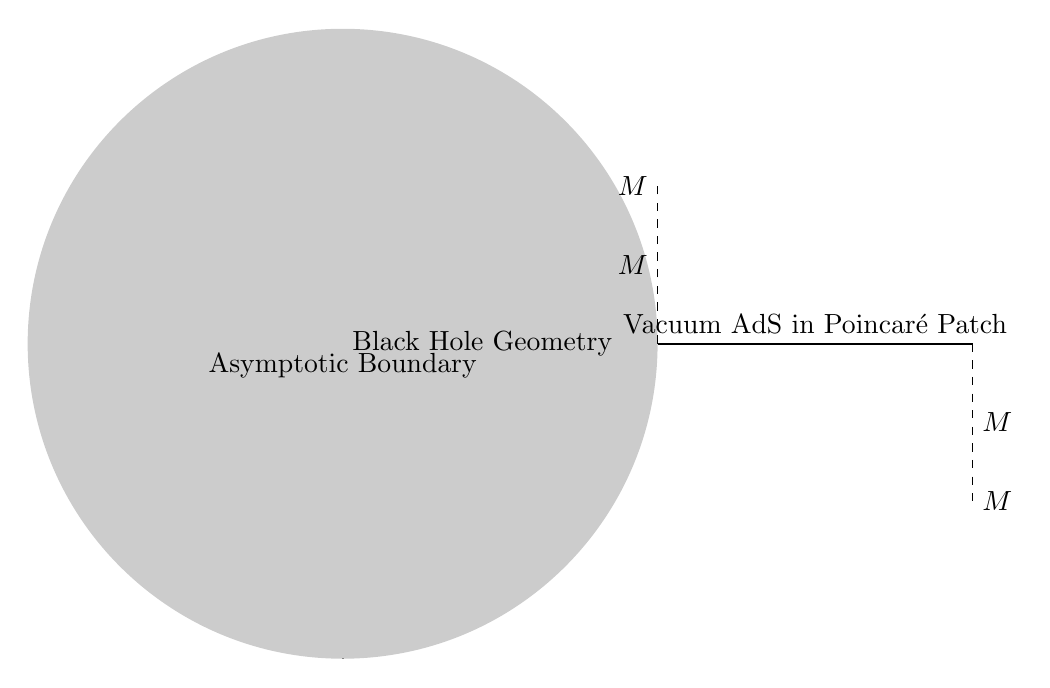
\begin{tikzpicture}[scale=2, x=1cm, y=1cm]

    % Asymptotic Boundary (Right Side)
    \draw[thick, dashed] (-3, -2) -- (-3, 2);
    
    % Black Hole Geometry (Outside Mass Shell)
    \fill[gray!40] (-3, 0) circle (2);
    
    % Vacuum AdS in Poincaré Patch (Inside Mass Shell)
    \draw[thick] (-1, 0) -- (1, 0);
    \draw[dashed] (-1, 0) -- (-1, 1) node[midway, left] {$M$};
    \draw[dashed] (1, 0) -- (1, -1) node[midway, right] {$M$};
    
    % Labels
    \node at (-3, 0) [below] {Asymptotic Boundary};
    \node at (-3, 0) [right] {Black Hole Geometry};
    \node at (0, 0) [above] {Vacuum AdS in Poincaré Patch};
    \node at (-1, 1) [left] {$M$};
    \node at (1, -1) [right] {$M$};

\end{tikzpicture}
\end{document}